\documentclass{article}

\usepackage{graphicx}
\usepackage{tikz}
\usepackage{tikzsymbols}
\usetikzlibrary{calc,patterns,shapes.geometric}
\pagestyle{empty}
\usepackage[margin=0pt]{geometry}
\geometry{papersize={14in,12in}}

\def\centerarc[#1](#2)(#3:#4:#5){\draw[#1] ($(#2)+({#5*cos(#3)},{#5*sin(#3)})$) arc (#3:#4:#5);}

\begin{document}
	\begin{figure}
		\centering
		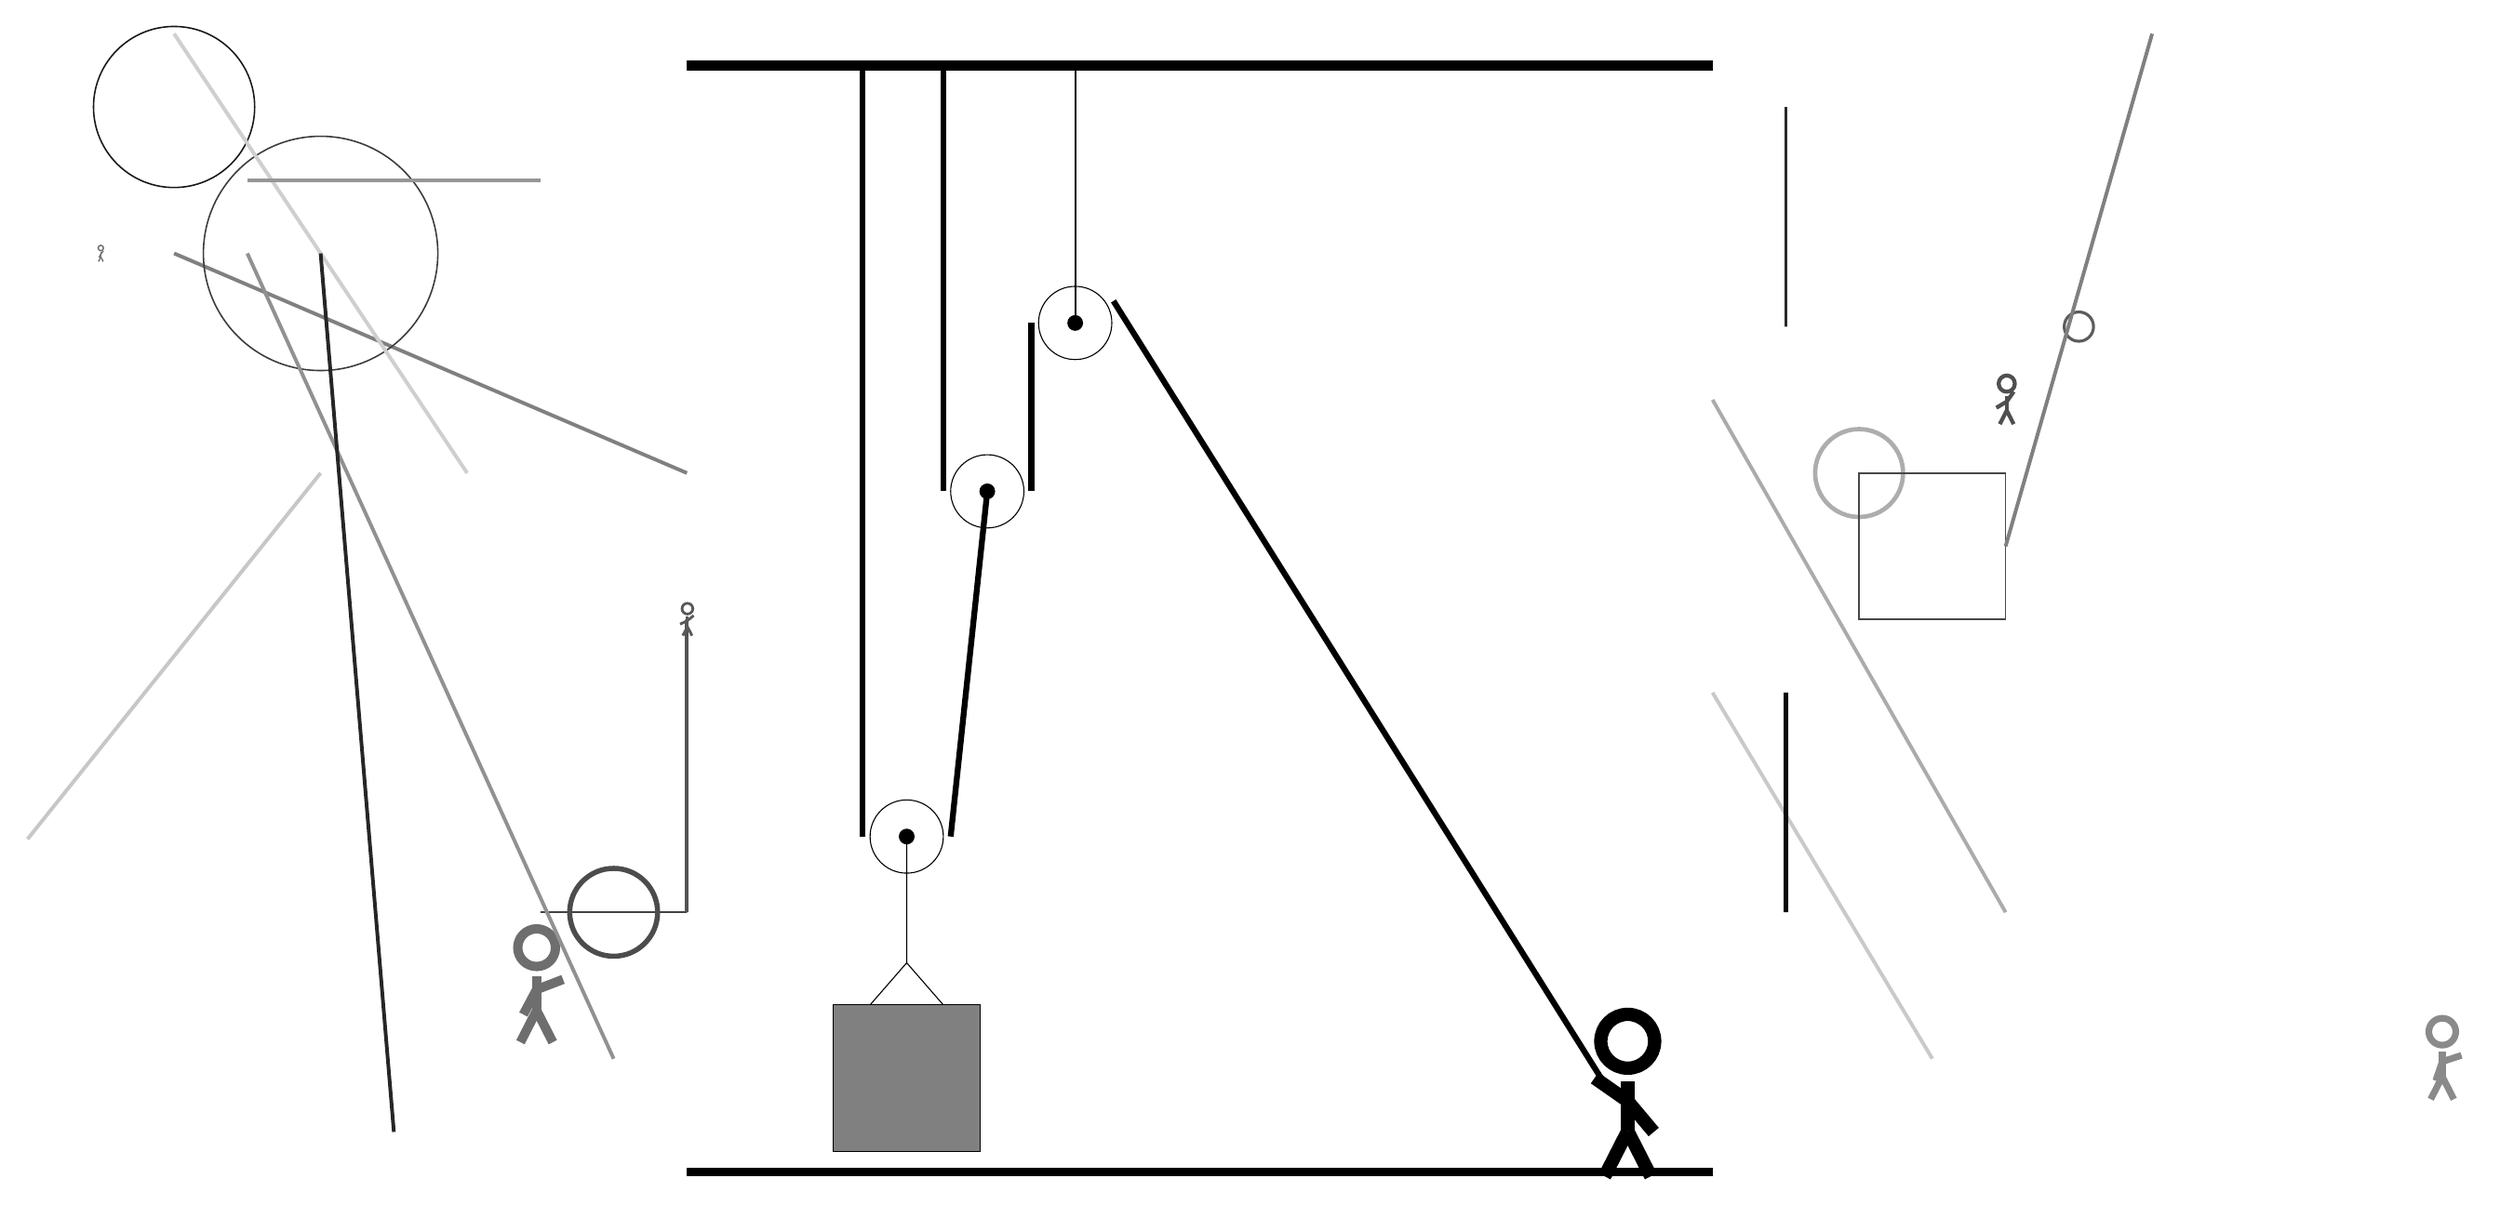
\begin{tikzpicture}
			%%%%% START %%%%%
			
			\draw[fill=black] (-2, 11.5) rectangle (12, 11.625);
			
			\draw (1, 1.035) circle (0.5);
			\draw[fill=black] (1, 1.035) circle (0.1);
			
			\draw (2.1, 5.75) circle (0.5);
			\draw[fill=black] (2.1, 5.75) circle (0.1);
			
			\draw (3.3, 8.05) circle (0.5);
			\draw[fill=black] (3.3, 8.05) circle (0.1);
			\draw[thick] (3.3, 8.05) -- (3.3, 11.5);
			
			\draw (1, 1.035) -- (1, -0.69) -- (0.5, -1.265) -- (1.5, -1.265) -- (1, -0.69);
			\draw[fill=black!50] (0, -1.265) rectangle (2, -3.265);
			
			\draw[line width=0.8mm] (0.4, 11.5) -- (0.4, 1.035);
			\centerarc[line width=0.8mm](1, 1.035)(180:360:0.6);
			\draw[line width=0.8mm](1.6, 1.035) -- (2.1, 5.75);
			\draw[line width=0.8mm] (1.5, 11.5) -- (1.5, 5.75);
			\centerarc[line width=0.8mm](2.1, 5.75)(180:360:0.6);
			\draw[line width=0.8mm](2.7, 5.75) -- (2.7, 8.05);
			\centerarc[line width=0.8mm](3.3, 8.05)(30:180:0.6);
			\draw[line width=0.8mm] (3.822, 8.35) -- (10.5, -2.3);
			
			\node at (10.8, -2.5) {\Strichmaxerl[10][-35][-50]};
			
			\draw [line width=0.6mm, color=black!32](14, 6) circle (0.6);
			
			\draw[line width=0.2mm, color=black!74] (-4, 0) rectangle (-2, 0);
			\draw[line width=0.5mm, color=black!50](-2, 6) -- (-9, 9);
			\node[line width=0.5mm, color=black!69] at (16, 7) {\Strichmaxerl[3][31][55]};
			\draw[line width=0.5mm, color=black!67] (-2, 4) rectangle (-2, 0);
			
			\draw [line width=0.2mm, color=black!77](-7, 9) circle (1.6);
			
			\draw [line width=0.2mm, color=black!91](-9, 11) circle (1.1);
			\node[line width=0.2mm, color=black!57] at (-4, -1) {\Strichmaxerl[7][62][21]};
			\draw[line width=0.5mm, color=black!21](15, -2) -- (12, 3);
			\draw[line width=0.5mm, color=black!22](-7, 6) -- (-11, 1);
			\draw[line width=0.5mm, color=black!33](12, 7) -- (16, 0);
			\draw[line width=0.5mm, color=black!19](-5, 6) -- (-9, 12);
			\node[line width=0.4mm, color=black!46] at (22, -2) {\Strichmaxerl[5][71][18]};
			
			\draw[line width=0.3mm, color=black!84] (13, 11) rectangle (13, 8);
			\node[line width=0.7mm, color=black!57] at (-10, 9) {\Strichmaxerl[1][64][51]};
			\draw[line width=0.5mm, color=black!43](-3, -2) -- (-8, 9);
			
			\draw[line width=0.5mm, color=black!41](-4, 10) -- (-8, 10);
			\draw [line width=0.4mm, color=black!64](17, 8) circle (0.2);
			\draw[line width=0.2mm, color=black!72] (14, 6) rectangle (16, 4);
			\draw [line width=0.7mm, color=black!70](-3, 0) circle (0.6);
			\node[line width=0.3mm, color=black!65] at (-2, 4) {\Strichmaxerl[2][26][39]};
			\draw[line width=0.5mm, color=black!85](-7, 9) -- (-6, -3);
			\draw[line width=0.5mm, color=black!50](16, 5) -- (18, 12);
			\draw[line width=0.6mm, color=black!97] (13, 0) rectangle (13, 3);
			
			\draw[fill=black] (-2, -3.5) rectangle (12, -3.6);
			
			%%%%% END %%%%%
		\end{tikzpicture}
	\end{figure}	
\end{document}